\section{Implementierung}
Dieses Kapitel beschreibt die Umsetzung des Projekts im Detail. Es wird ein Überblick über den Implementierungsprozesse gegeben, der Vorgehensweise bei der Entwicklung und ein Einblick in Probleme, welche während der Entwicklung aufgetreten sind.
Neben einer schrittweisen Darstellung der Implementierung werden auch exemplarisch Codebeispiele vorgestellt.
\subsection[Implementierungsdetails]{Implementierungsdetails}
In den Implementieungsdetails werden die Vorgehensweisen und Konzepte, welche für die Implementierung des Fontends und Backends benötigt werden, erläutert.

\subsubsection[Frontend]{Frontend}
Das \gls{sapui5}-Framework verwendet zur Darstellung der Seiten sogenannte \textit{Views} welche in \gls{xml} Dateien definiert werden.
Diese Views müssen mit der Dateiendung \textbf{.view.xml} enden, damit sie von \gls{sapui5} als View erkannt werden.

Views sind eine Art Kontainer für \gls{sapui5}-Elemente (Buttons, Input Felder, Tabellen, Listen, ...) und \gls{sapui5}-Layouts (Flex Box, HBox, VBox).
Views können jedoch auch andere Views beinhalten und so einen verschachtelten Aufbau der Seite schaffen.
Die \gls{sapui5}-Elemente sind vorgefertigte Komponenten welche von \gls{sapui5} bereitgestellt werden, um eine einheitliche Benutzeroberfläche zu schaffen, welche dann auch über verschiedene SAP-Anwendungen in einem Unternehmen konsistent ist.

Für die Admin-UI Seite sollen die Views und Komponenten wie in Abbildung \ref{fig:appstructure} angeortnent und strukturiert werden.
Die Unterseiten für die Eingabefelder aus den Anforderungen \ref{Tab:A4}, \ref{Tab:A5} und \ref{Tab:A6} werden in eigenen Views angezeigt, zwischen denen der Benutzer über die Navigationsleiste wechseln kann.

\begin{figure}[H]
    \centering
    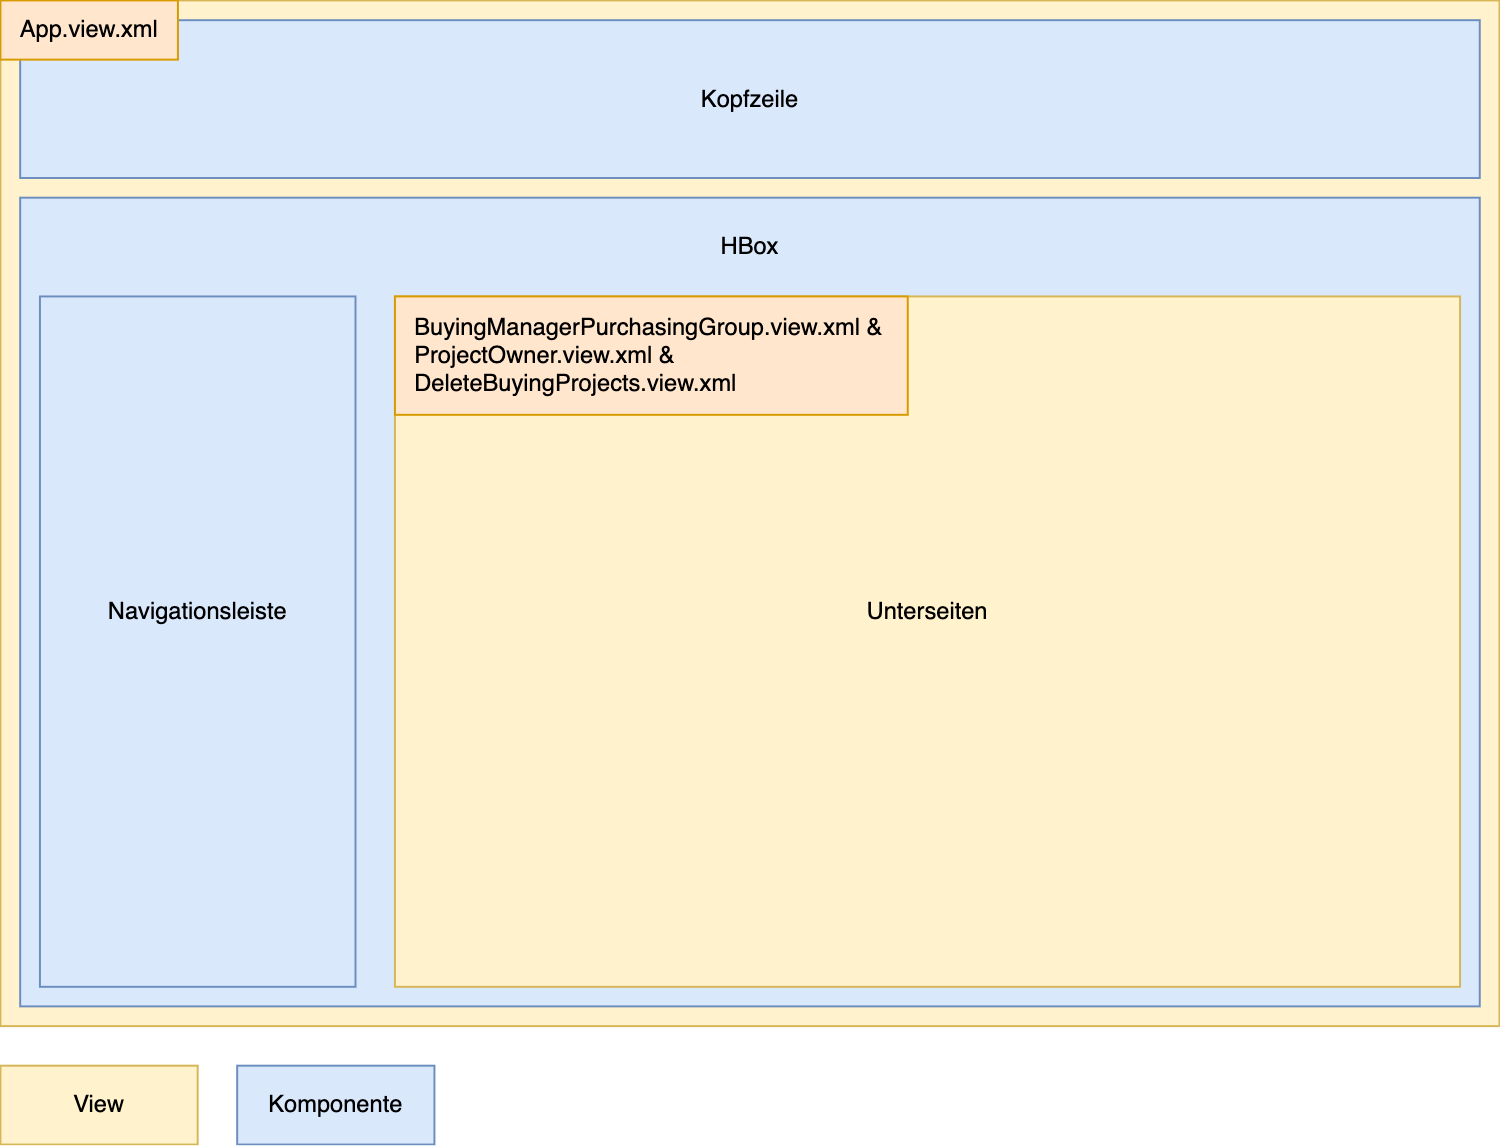
\includegraphics[width=\linewidth]{Images/AppStructure.png}
    \caption[Darstellung der Anwendungsstruktur]{Darstellung der Anwendungsstruktur}
    \label{fig:appstructure}
\end{figure}

Für jeden View kann ein \textit{Controller} erstellt werden, welcher die Funktionalität für die Views bereitstellt und Elemente dynamisch laden kann.
\subsection[Schrittweise Beschreibung der Implementierung]{Schrittweise Beschreibung der Implementierung}

\subsection[Codebeispiele und Erklärungen]{Codebeispiele und Erklärungen}

\subsection[Herausforderungen und Problemlösungen]{Herausforderungen und Problemlösungen}

\subsection[Darstellung aufgetretener Herausforderungen]{Darstellung aufgetretener Herausforderungen}

\subsection[Beschreibung der Lösungsansätze]{Beschreibung der Lösungsansätze}
